\section{Etat de l'art}
\graphicspath{ {./figuresState} }

Pour la mesure de l'humectation, deux grandes familles de capteurs existent. Les capteurs résistifs fonctionnent à l'aide de deux électrodes en peigne. Lorsqu'une goutte se forme entre deux doigts du peigne la résistance mesurée change. Cette technique est simple et peu coûteuse mais les gouttes doivent être suffisamment grosses pour toucher deux doigts du peigne. Pour contrer ce problème une peinture ou un papier absorbant est posé sur les électrodes. Ce procédé ajoute un problème de faux positif. La couche absorbe aussi l'humidité de l'air et le point de transition entre une feuille humide ou sèche est mal définie. Ces capteurs demandent une attention toute particulière à la calibration. Les couches absorbantes s'abîment vite et doivent être changées périodiquement. Davis\cite{davis}, SPECTRUM Technologies Inc.\cite{spectrum} et Caipos GmbH \cite{caipos} proposent ce type de capteur. Metos propose un capteur un peu similaire. A la place d'un peigne sous une surface absorbante, il n'a que deux électrodes à chaque extrémité de la surface. Le principe reste le même que pour les autres et souffrent des mêmes inconvénients.

\begin{figure}[!ht]
\centering
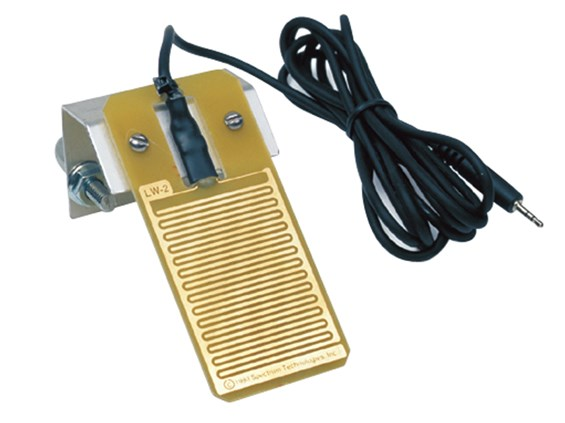
\includegraphics[width=8cm]{davis}
\caption{Capteur Résistif Davis \cite{davis}}
\end{figure}


La deuxième famille sont les capteurs capacitifs. Ils sont beaucoup moins répandu car plus complexe et plus chère. Un seul constructeur en commercialise. Meter \cite{meter} anciennement DECAGON produit le PHYTOS31. Ce même capteur est repris par plusieurs revendeurs qui l'intègrent dans leur écosystème. C'est par exemple le cas de EVVOS \cite{evvos}.



\begin{figure}[!ht]
\centering
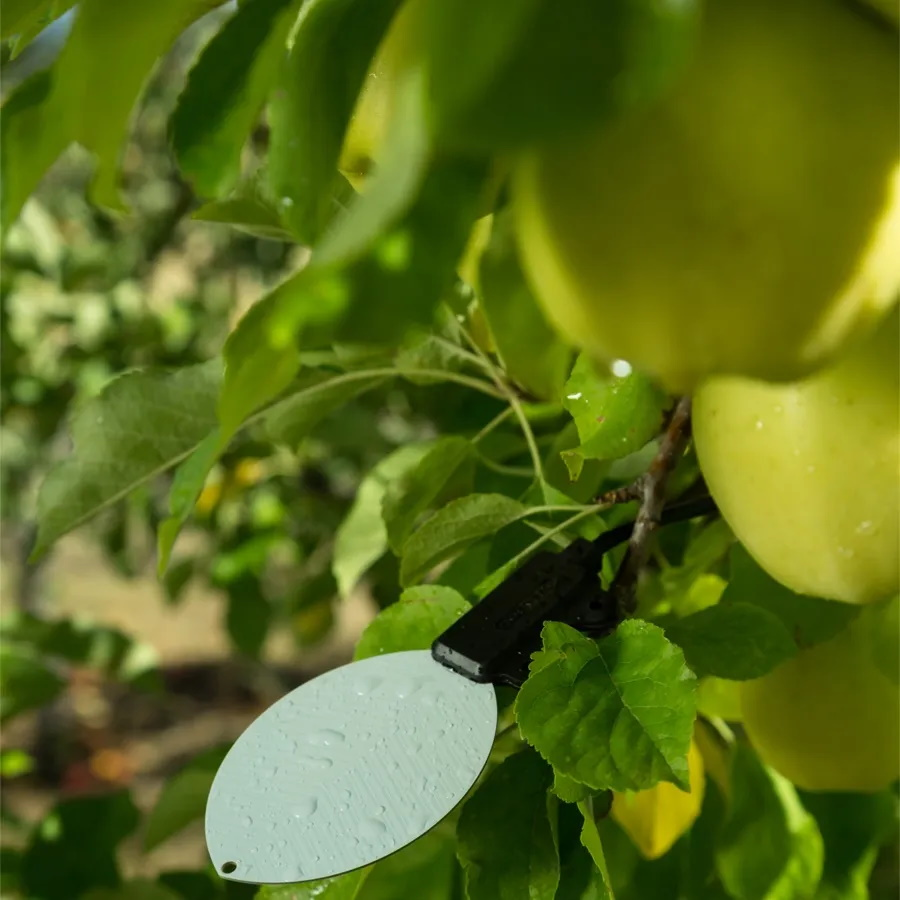
\includegraphics[width=8cm]{leaf-wetness-3}
\caption{Capteur capacitifs PHYTOS31 \cite{evvos}}
\end{figure}

\newpage
Les capteurs capacitifs utilisent aussi deux électrodes en peigne mais elles ne sont pas en contact direct avec l'eau. Elles sont protégées par une couche de résine imperméable qui reproduit la surface d'une feuille. La  capacité est mesurée entre les deux électrodes. La mesure utilise les propriétés diélectriques de l'eau et sa permittivité relative de 80. Lorsqu'une goutte se pose, la capacité augmente. Ce type de capteur n'a pas les désavantages des capteurs résistifs. Il n'a pas besoin d'être calibré à l'installation. Il est, par contre, plus complexe à développer avec la mesure de capacité. L'université polytechnique de Catalogne en Espagne a publié un article\cite{HORNERO2017286} dans lequel il développe un tel capteur avec comme objectif de créer une alternative bon marché. Ils ont réussi à obtenir un prototype convaincant.

Durant ce projet nous nous concentrerons sur un capteur capacitif. Ces avantages surpassent le fait qu'il soit plus complexe et plus coûteux à mettre en place. La mesure de capacité est très utilisé dans pleins d'autre type de capteurs. Les capteurs tactiles s’approchent par leur conception de ce que nous cherchons à atteindre. Ces capteurs utilisent le fait que le corps humain, dont les doigts, sont composé en majorité d'eau. Une variation de capacité est mesuré quand l'utilisateur pose son doigt sur un diélectrique. Plusieurs circuits intégrés sont utilisés par les capteurs tactiles par exemple le FDC1004 \cite{fdc1004}, le AD7745 \cite{ad7745},ou le AD7150 \cite{ad7150}. Pour mesurer la capacité, Ils appliquent un signal d'excitation sur un des pôle et mesurent la quantité de charge qui traverse à l'autre pôle à l'aide d'un convertisseur sigma delta du deuxième ordre. La capacité est ensuite converti en valeur numérique. Ces circuits pourraient être utilisé dans notre application.
